\chapter{曲率估计}
\section{逐点估计}
设$\Sigma^{n-1} \subset \M^n$是光滑子流形. $\vec{n}$是 $\Sigma$的单位法向. 设$T$是$(0,2)$型张量, $T=T_{ij}dx^idx^j$. 记号约定如下.
\begin{equation}
    (\nabla^2_{XY}T)(Z,W)=\nabla^2T(Z,W,Y,X).
\end{equation}
在局部坐标下,
\begin{equation}
    \nabla^2_{lk}T_{ij}=(\nabla^2_{\partial l,\partial k}T)(\PI,\PJ)=\nabla^2T(\PI,\PJ, \partial k,\partial l)=T_{ijkl}.
\end{equation}
Codazzi方程.
\begin{equation}
    R^\M(X,Y,W,\vec{n}) = \nabla \II(W,Y,X) - \nabla \II (W,X,Y).
\end{equation}
Gauss方程
\begin{equation}
    R^\M(X,Y,Z,W) = R^\Sigma(X,Y,Z,W)-\II(X,W)\II(Y,Z)+\II(X,Z)\II(Y,W).
\end{equation}
求导交换次序.
\begin{equation}
    \nabla^2_{X,Y}T(Z,W) = \nabla^2_{Y,X}T(Z,W)-T(R(X,Y)Z,W)-T(Z,R(X,Y)W).
\end{equation}
在局部坐标下,
\begin{equation}
    T_{ijkl}=T_{ijlk}-R_{lki}^pT_{pj}-R_{lkj}^pT_{ip}.
\end{equation}
求导交换次序的结果可以参考\cite[定理7.14]{lee}. 需要注意, $T_{ijkl}=(\nabla^2_{lk}T)(\PI,\PJ)$.  
\begin{proposition}
    设$\Sigma^{n-1} \subset \R^n$是光滑曲面. $\nabla, \Delta$为$\Sigma$上的算子. $\II$为其第二基本型, $H$是平均曲率. 则
    \begin{equation} \label{simon1}
        \Delta \II_{ij}=\nabla^2_{ij}H + Hg^{kl}\II_{ik}\II_{jl}-\abs{\II}^2\II_{ij}.
    \end{equation}
\end{proposition}
\begin{proof}
    固定点$p$, 选取$p$点附近的测地坐标, 则有
    \begin{equation}
        \Delta \II_{ij}=\II_{ij;kk}=\II_{ik;jk}=\II_{ik;kj}-R_{kji}^p\II_{pk}-R_{kjk}^p\II_{ip}.
    \end{equation}
    而
    \begin{equation}
        \II_{ik;kj}=\II_{kk;ij}=H_{ij}.
    \end{equation}
    \begin{equation}
        \begin{split}
            R_{kji}^p\II_{pk}+R_{kjk}^p\II_{ip} &= R_{kjip}\II_{pk}+R_{kjkp}\II_{ip}\\
            &=\II_{kp}\II_{ji}\II_{kp}-\II_{ki}\II_{jp}\II_{pk}+\II_{kp}\II_{jk}\II_{ip}-\II_{kk}\II_{jp}\II_{ip} \\
            &=\abs{\II}^2\II_{ij}-Hg^{pq}\II_{jp}\II_{iq}
        \end{split}
    \end{equation}
\end{proof}
\begin{proposition}[Simons等式] \label{simon_equation}
    设$\Sigma^{n-1}$是极小曲面, 则有
    \begin{equation}
        \Delta\abs{\II}^2 = 2(\abs{\nabla \II}^2-\abs{\II}^4).
    \end{equation}
\end{proposition}
\begin{proof}
    将等式\eqref{simon1}写成坐标无关的形式, 又因$\Sigma$是极小曲面, 则有
    \begin{equation}
        \Delta \II = -\abs{\II}^2 \II
    \end{equation}
    由于$\Tr$与联络导数可交换, 则
    \begin{equation}
        \begin{split}
            \Delta \abs{\II}^2 = \Delta (\Tr^2(\II\otimes\II)) &= \Tr^2(\Delta \II \otimes\II + \II \otimes \Delta \II + 2 \Tr(\nabla \II, \nabla \II)) \\
            &=\Tr^2(-2\abs{\II}^2 \II\otimes\II+2\Tr(\nabla \II \otimes \nabla \II)) \\
            &=-2\abs{\II}^4+2\abs{\nabla \II}^2.
        \end{split}
    \end{equation}
\end{proof}
\begin{proposition}[Simons不等式]
    设$\Sigma^{n-1}$是极小曲面, $\nabla,\Delta$为$\Sigma$上的算子. 则
    \begin{equation} \label{simon_inequality}
        \Delta \abs{\II}^2 \ge -2\abs{\II}^4+2(1+\frac{2}{n-1})\abs{\nabla \abs{\II}}^2.
    \end{equation}
\end{proposition}
\begin{proof}
    证明与命题\eqref{kato}类似. 我们首先来计算 $\abs{\nabla \abs{\II}}^2$. 固定点$p$, 取$p$点处的测地坐标使得$\II=diag(\lambda_i)$.
    \begin{equation} \label{s11}
        \begin{split}
            \abs{\nabla \abs{\II}}^2 = \frac{\abs{\inner{\nabla \II}{\II}}^2}{\abs{\II}} &= \frac{\sum_j(\sum_i\lambda_i\II_{iij})^2}{\sum_i\lambda_i^2} \\
            &\le \sum_{ji}\II_{iij}^2
        \end{split}
    \end{equation}
    而
    \begin{equation} \label{s12}
        \begin{split}
            \sum_{ji}\II_{iij}^2 &= \sum_{j\ne i}\II_{iij}^2+ \sum_{i}\II_{iii}^2 \\
            &= \sum_{j\ne i}\II_{iij}^2+ \sum_{i}(-\sum^{n-1}_{j \ne i}\II_{jji})^2\\
            &\le \sum_{j\ne i}\II_{iij}^2+ \sum_{i}(n-2)\sum_{j\ne i}\II_{jji}^2\\
            &\le (n-1)\sum_{j\ne i}\II_{iij}^2\\
            &= \frac{n-1}{2}(\sum_{j\ne i}\II_{iji}^2 +\sum_{j\ne i}\II_{jii}^2)
        \end{split}
    \end{equation}
    \eqref{s12}两侧同乘以$\frac{2}{n-1}$后与\eqref{s11}相加可得,
    \begin{equation}
        \begin{split}
            \abs{\nabla \abs{\II}}^2+\frac{2}{n-1} \abs{\nabla \abs{\II}}^2 &\le \sum_{ji}\II_{iij}^2 + \sum_{j\ne i}\II_{iji}^2 +\sum_{j\ne i}\II_{jii}^2 \\
            &\le \sum_{ijk}\II^2_{ijk}
        \end{split}
    \end{equation}
    再由Simon等式\eqref{simon_equation}即可得到不等式\eqref{simon_inequality}.
\end{proof}
\begin{theorem}\label{choi_schoen}
    设$\Sigma^2 \subset \R^3$是极小曲面.  则存在常数$\epsilon, \rho>0$, 使得 $\forall p \in \Sigma, r_0 < \rho$, 如果
    \begin{enumerate}
        \item $\partial \Sigma \cap B_{r_0}(p)=\emptyset$.
        \item $\int_{\Sigma \cap B_{r_0}} \abs{\II}^2\le \epsilon$.
    \end{enumerate}
    那么$\forall  0 < \sigma \le r_0$及$y \in B_{r_0-\sigma}$, 成立
    \begin{equation}
        \sigma^2 \abs{\II}^2(y) \le \delta, \text{ here }\delta= \frac{\int_{\Sigma \cap B_{r_0}}\abs{\II}^2}{\epsilon}.
    \end{equation}
\end{theorem}
\begin{proof}
    将$B_{r_0}$简写为$B$. 只需要证明$F(x)=d^2(x,\P B)\abs{\II}^2(x) \le \delta$即可. 我们用反证法. 设$F$在$q$点处取到最大值$\max_{x \in B}F(x)$. 注意到在$\partial B$上, $F(x) \eq 0$. 则$q$是内点.  设$F(q) > \delta$, 我们将证明当$\epsilon$足够小时, 会推出一个矛盾. 取 $\lambda$使得
    \begin{equation}
        \lambda^2\abs{\II}^2(q)=\frac{\delta}{4} \le \frac{1}{4} d^2(q,\P B)\abs{\II}^2(q).
    \end{equation}
    因此, 有
    \begin{equation}
        \lambda \le \frac{1}{2}d(q,\P B).
    \end{equation}
    由三角不等式可知,  $\forall y \in B_\lambda(q)$,
    \begin{equation}
        \frac{1}{2} \le \frac{d(y,\P B)}{d(q,\P B)} \le 2.
    \end{equation}
    于是
    \begin{equation}
        \begin{split}
            \sup_{y\in B_\lambda(q)} d^2(q,\P B) \abs{\II}^2(y) \le &4\sup_{y\in B_\lambda(q)}d^2(y,\P B)\abs{\II}^2(y) \\
            =& 4d^2(q,\P B) \abs{\II}^2(q).
        \end{split}
    \end{equation}
    因此,
    \begin{equation}
        \sup_{y \in B_\lambda(q)} \abs{\II}^2(y) \le 4\abs{\II}^2(q)=\frac{\delta}{\lambda^2}.
    \end{equation}
    通过变换$x\to \lambda x$, 上面的不等式变为
    \begin{equation} \label{ii_sup}
        \sup_{y \in B_1(q)} \abs{\II}^2(y) \le 4\abs{\II}^2(q)=\delta \le 1.
    \end{equation}
    由Simons不等式, 我们得到
    \begin{equation}
        \Delta \abs{\II}^2 \ge -2\abs{\II}^4 \ge -2 \abs{\II}^2.
    \end{equation}
    由推论\eqref{sub_harmonic}(取$s=1,\lambda=2$)可知,
    \begin{equation}
        \frac{\delta}{4}=\abs{\II}^2(q) \le C \int_{B_1} \abs{\II}^2 \le C\delta\epsilon.
    \end{equation}
    则当$\epsilon$足够小时, 显然是不可能的.
\end{proof}
\begin{remark}
    上面的证明在黎曼流形上也成立.  在$\R^3$中, 由于$d(x,\P B)\abs{\II(x)}$的伸缩不变性, 实际上$r \le \rho$的条件并不需要.
\end{remark}
把定理\eqref{choi_schoen}写成下面形式往往是方便的.
\begin{theorem*}\label{choi_schoen_cor}
    设$\Sigma^2 \subset \R^3$是极小曲面.  则存在常数$\epsilon, \rho>0$, 使得 $\forall r_0 < \rho$, 如果
    \begin{enumerate}
        \item $\partial \Sigma \cap B_{r_0}(p)=\emptyset$.
        \item $\int_{\Sigma \cap B_{r_0}} \abs{\II}^2\le \epsilon$.
    \end{enumerate}
    那么
    \begin{equation}
        \mathop{\sup}_{B_{\frac{r_0}{2}}}\abs{\II(x)} \le \frac{C}{r_0}.
    \end{equation}
\end{theorem*}

\begin{lemma}[一致图像引理] \label{uniform_graph}
    设$\Omega \subset \R^3$是具有光滑边界的开集. 设$\Sigma^2 \subset \Omega$是嵌入的光滑曲面, 并且$\Sigma$在$\Omega$中是闭的. 设$\abs{\II} \le C$. 则$\Sigma$可以局部一致地表示成函数图像的形式. 确切地说, $\forall p \in \Sigma$, $R\in (0,R_0)$. 这里, 
    \begin{equation}
        R_0=\min\{\frac{1}{4C}, \frac{1}{2}d(p,\partial \Omega)\}.
    \end{equation}
    设$D(p,R)$为$T_p\Sigma$上以$p$为中心, 半径为$R$ 圆盘, $W(p,R)=D(p,R)\times \R$. 
    \begin{align}
        &D(p,R)= \{p+\vec{v}\mid v \in T_p\Sigma, \abs{v} < R\}.  \\
        &W(p,R)= \{q+t\vec{n}(p)\mid q \in D(p,R), t \in \R\}.
    \end{align}
    则存在函数$u: D(p,R)\to \R$ 使得$u(p)=0$, 并且$\Sigma$可以写成$u$的在$D(p,R)$上的图像的形式. 并且, 给定$q \in D(p,R)$,
    \begin{enumerate}
        \item $\abs{u(p)-u(q)} \le 8C\abs{p-q}$.
        \item $\abs{\nabla u}(q) \le 8C\abs{p-q}$.
        \item $\abs{\nabla^2 u}(q) \le 16C$.
    \end{enumerate}
\end{lemma}
\begin{remark}
    一致图像引理不要求曲面是极小的.
\end{remark}
\begin{proof}
    设$\Sigma_{p,r}$是$\Sigma \cap W(p,r)$的包含$p$点的连通分支.  经过旋转平移之后, 设$p =0, T_p\Sigma = \{z=0\}$. 设$R \in \R$满足以下条件, 并且取上界: $\Sigma_{p,R}$可以表示为某个函数$u \in C^\infty(D(p,R))$的图像, $u(0)=0, \nabla u(p)=0$ 且 $\abs{\nabla u} \le 1$. 注意, $\abs{\nabla u} \le 1$等价于$N_3=\inner{\vec{n}}{e_3}=\frac{1}{\sqrt{1+\abs{Du}^2}} \ge \frac{1}{2}$. 现在, 当$R$变得更大一点时, 有两种情况可能发生:
    \begin{enumerate}
        \item 函数$u$可以光滑地延拓到$D(p,R)$的邻域内, 但是会导致$N_3< \frac{1}{2}$. \label{case1}
        \item 函数$u$不能继续延拓, 这表明$\G(u)$碰到了$\Omega$的边界. \label{case2}
    \end{enumerate}
    直接计算可知, 我们有如下的比较关系
    \begin{equation}
        \frac{\abs{\nabla^2 u}^2}{(1+\abs{\nabla u}^2)^3} \le \abs{\II}^2 \le 2 \frac{\abs{\nabla^2 u}^2}{1+\abs{\nabla u}^2}.
    \end{equation}
    在$D(p,R)$上, 由于$\abs{Du} \le 1$, 则
    \begin{equation}
        C^2 \le \abs{\nabla^2 u} \le 8C^2.
    \end{equation}
    现在, 设情况\eqref{case1}发生, 设$q \in \partial D(p,R)$使得$\abs{\nabla u(q)}=\frac{1}{2}$. 则
    \begin{equation}
        1=\abs{\nabla u(0)-\nabla u(q)} \le \abs{\nabla^2 u}\abs{q}\le 4CR.
    \end{equation}
    因此, $R \ge \frac{1}{4C}$.
    若情况\eqref{case2}发生,  设$Q=(q,u(q))\in \partial \Omega, q \in \partial D(p,R)$. 设$\alpha$是连接 $p,q$的线段, 则
    \begin{equation}
        d(p,Q) \le \sup \sqrt{1+\abs{\nabla u}}l_\alpha \le 2R.
    \end{equation}
    即有$R \ge \frac{1}{2}{d(p,\partial \Omega)}$.  其余性质均可由中值定理得到.
\end{proof}
\begin{corollary} \label{choi_schoen_intrinsic}
    定理\eqref{choi_schoen}中的$B_r$可以换成$B^\Sigma_r$.
\end{corollary}
\begin{proof}
    在定理\eqref{choi_schoen}的证明中, 有了不等式\eqref{ii_sup}(欧氏度量换成内蕴度量后, 直到这里的推导都是正确的), 我们就可以用应用一致图像引理. 由于此时$\abs{\nabla u}$一致有界, 那么$\Sigma$上的内蕴度量与外蕴度量实际上是局部可比较的. 最后在$B_\frac{1}{4}$(引理\eqref{uniform_graph}中, $C=1$)上应用推论\eqref{sub_harmonic}.
\end{proof}

\begin{theorem} \label{compactness}
    设$\{\Sigma_i \} \subset \R^3$是完备极小曲面. 设$p_i \in \Sigma_i$且$p_i \to p$.  设存在常数$C$使得$\forall i$,
    \begin{equation}
        \abs{\II_{\Sigma_i}} \le C.
    \end{equation}
    则存在子列$\Sigma_{i_k}$及极小曲面$\Sigma$使得$\Sigma_{i_k} \overset{C^\infty}{\longrightarrow} \Sigma$.
\end{theorem}
\begin{proof}
    在$p$点处, (选取子列)设$T_{p_k}\Sigma_k \to \{z=0\}$.  设$B_\delta(0)=\{(x,y,z)\mid z=0, x^2+y^2 \le \delta^2\}$. 由一致图像引理, 存在$\delta=\delta(C)>0$使得$\Sigma_k$可以表示成为$B_\delta(0)$上的函数$u_k$的图像, 且在$B_\delta$上, $Du_k$一致有界. 则存在函数$u$使得 $u_k \to u$. 由Schauder估计可知, $u_k \overset{C^\infty}{\longrightarrow} u$.  
    \par 取$p \in \P B_\delta(0)$, 则在$p$点的$\delta$邻域中,  重复上面的过程. 我们可以得到在更大区域上的收敛子列.  此过程可以一直继续下去, 直到我们得到完备的极小曲面.
\end{proof}
在后面的曲率估计中, 下面的引理将会被频繁用到.
\begin{lemma}
    设$\Sigma \subset \R^3$是嵌入的光滑曲面. 则
    \begin{equation}
        d(x,\P \Sigma)\abs{\II(x)},\s  \int_\Sigma \abs{\II}^2dv_g
    \end{equation}
    是在伸缩变换下的不变量.
\end{lemma}
\begin{theorem}
    存在常数$C>0$使得对于任意定向的稳定极小曲面$\Sigma^2 \subset \R^3$, 成立
    \begin{equation}
        d_\Sigma(x,\P \Sigma)\abs{\II}(x)  \le C.
    \end{equation}
\end{theorem}
\begin{proof}
    反证法. 设存在稳定极小曲面$\Sigma_k$及$p_k \in \Sigma_k$使得
    \begin{equation}
        d(p_k, \P \Sigma_k)\abs{\II_k(p_k)}  \to \infty.
    \end{equation}
    如果$\Sigma_k$是无界的, 则截断$\Sigma_k$使其是带有光滑边界的紧集. 不失一般性, 设$p_k$取到$d(x,\P \Sigma_k)\abs{\II_k(x)}$的最大值. 经过平移旋转后, 设 $p_k$在0点处. 对$\Sigma_k$做伸缩变换$ x \to \abs{\II_k(p_k)}x$, 得到新的极小曲面列, 仍记为 $\Sigma_k$. 这些新的极小曲面仍然满足: $\Sigma_k$是稳定的, 并且$d(0, \P \Sigma_k)\abs{\II_k(0)} \to \infty$. 另外,  $\abs{\II_k(0)}=1$. 因此, $d(0, \P \Sigma_k) \to \infty$. 根据$p_k$的选取, $\forall x \in \Sigma_k$,
    \begin{equation}
        d(x,\P \Sigma_k)\abs{\II_k(x)} \le d(0,\P \Sigma_k).
    \end{equation}
    设$x \in B_r$. 则
    \begin{equation}
        \abs{\II_k(x)} \le \frac{d(0,\P \Sigma_k)}{d(x,\P \Sigma_k)} \to 1.
    \end{equation}
    因此, $\abs{\II_k}$局部一致有界. 根据定理\eqref{compactness}, 存在极小曲面$\Sigma$使得$\Sigma_k \overset{C^\infty}{\longrightarrow} \Sigma$. 显然$\Sigma$是完备的, 且$\abs{\II(0)}=1$. 下面我们说明$\Sigma$是稳定的.  否则的话, 存在$\Omega \subsub \Sigma$使得$\lambda_1(\L_\Sigma,\Omega) < 0$. 而由于$\Sigma_k \overset{C^\infty}{\longrightarrow} \Sigma$, $\L_{\Sigma_k} \to \L_\Sigma$, 则$\Sigma$是稳定的. 而由定理\eqref{stable_flat}可知, $\Sigma$是平面, 而这与$\abs{\II(0)}=1$矛盾.
\end{proof}
%\begin{proof}
%    记$r_0=d(x,\partial \Sigma)$. 由命题\eqref{mc_area}可知, $\forall 0<r < r_0$, 
%    \begin{equation}
%        \Area(B^\Sigma_r) \le Cr^2.
%    \end{equation}
%    (这里如果$B^\Sigma_r$不是嵌入圆盘, 我们就在万有覆盖中来做). 固定$x$, 设$r=d(y,x)$, 定义截断函数
%    \begin{equation}
%        \eta(y)=\left\{
%            \begin{aligned}
%                & 1, r\le e^{-N}r_0, \\
%                & \frac{\log r_0-\log r}{N}, e^{-N}r_0 < r < r_0, \\
%                & 0, r>r_0.
%            \end{aligned}
%        \right.
%    \end{equation}
%    由于$\abs{\nabla r}=1$, 则$\abs{\nabla \eta} \le \frac{1}{Nr}$. 将$\eta$代入到稳定性不等式中, 得到
%    \begin{equation}
%        \begin{split}
%            \int_{B^\Sigma_{e^-Nr_0}}\abs{\II}^2 \le \int_\Sigma \eta^2 \abs{\II}^2 &\le \int_\Sigma \abs{\nabla \eta}^2  \\
%            &\le \frac{1}{N^2}\sum_{i=-n}^{-1}\int_{B_{e^{i+1}r_0}^\Sigma-B_{e^ir_0}^\Sigma}\frac{1}{r^2} \\
%            &\le \frac{4\pi e^2}{3N}.
%        \end{split}
%    \end{equation}
%    $N$取足够大时就可以应用定理\eqref{choi_schoen}(推论\eqref{choi_schoen_intrinsic}).
%\end{proof}
\begin{theorem} \label{curvature_estimate_4pi}
    设$C \in (0,8\pi)$. 则存在常数$C_0=C_0(C)$使得: 如果$\Sigma \subset \R^3$是定向极小曲面, 并且
    \begin{equation}
        \int_\Sigma \abs{\II}^2 dv_g \le C.
    \end{equation}
    则$\forall x \in \Sigma$,
    \begin{equation}
        d(x,\P \Sigma)\abs{\II(x)} \le C_0.
    \end{equation}
\end{theorem}
定理\eqref{curvature_estimate_4pi}的证明需要下面的定理\eqref{total_curvature}.
\begin{theorem}\label{total_curvature}
    设$\Sigma^2$是非紧, 可定向, 完备的2维黎曼流形, 并且
    \begin{equation}
        \int_\Sigma K^- < +\infty. 
    \end{equation}
    这里, $K^-=-\min(K,0)$, $K$是Gauss曲率. 则有
    \begin{enumerate}
        \item $\int_\Sigma \abs{K} dv_g < +\infty$.
        \item 存在闭黎曼面$\mathcal{S}$及$\{p_1,p_2\cdots p_k\} \subset \mathcal{S}$使得$\Sigma$共形同构于$\mathcal{S}-\{p_i\}$.
    \end{enumerate}
    如果$\Sigma \subset \R^3$是极小曲面, 则
    \begin{enumerate}
        \item[3.] 存在整数$m \le 0$(可以为$-\infty$)使得 $\int_\Sigma K dv_g = 4m\pi$.
    \end{enumerate}
\end{theorem}
\begin{proof}
    设$p \in \Sigma$. 记$D_r=D(p,r)=\{x\in \Sigma \mid d_\Sigma(p,x) \le r\}$, 则$\P D_r$是分段光滑曲线. 设$\{\theta^r_i\}$是$\P D$上的非光滑点处的外角, 如是图所示.
    \begin{figure}[ht]
        \centering
        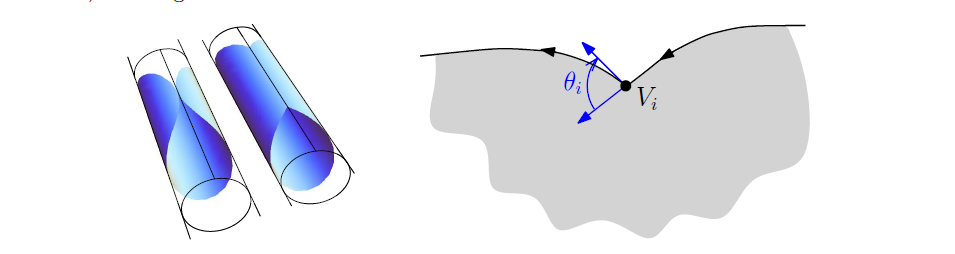
\includegraphics[scale=0.8]{images/angle.png}
        \caption{区域$D_r$的边界.}
        \label{angle}
    \end{figure}
    我们这里选取的定向使得$-\pi \le \theta_i \le 0$.  记$l(r)=l(\P D_r)$. 则由第一变分公式(非光滑点附近需要单独处理, 参考\cite{White}及\cite{Perez}),
    \begin{equation}
        l'(r)=\int_{\P D_r}K_{\P D}ds+2\sum \tan(\frac{\theta_i}{2}).
    \end{equation}
    而由于$\tan(\frac{\theta_i}{2}) \le \frac{\theta_i}{2}$, 及Gauss-Bonnet公式(分段光滑区域上的Gauss-Bonnet公式参考\cite{lee}),
    \begin{equation}
        l'(r)\le \int_{\P D_r}K_{\P D}ds+\sum \theta_i = 2\pi\chi(D_r)-\int_{D_r}Kdv_g.
    \end{equation}
    由于$\mathop{\limsup} l'(r) \ge 0$(若$ \mathop{\limsup l'(r)} \le \alpha <0$, 则存在$r$足够大使得$l(r) < 0$, 这是不可能的), 则有
    \begin{equation} \label{basic_inequality}
        \begin{split}
            0 &\le \limsup_{r\to \infty} l'(r) \le \limsup(2\pi \chi(D_r) - \int_{D_r}Kdv_g) \\
            & \le \limsup (2\pi(2-2p(D_r)-(\P D_r)^\#)-\int_{D_r}K^+dv_g+\int_{D_r}K^-dv_g)
        \end{split}
    \end{equation}
    其中, $p$为$D_r$的亏格, $(\P D_r)^\#$为$D_r$的边界的连通分支数. 上述不等式意味着, 存在常数$C$使得
    \begin{enumerate}
        \item $p(D_r), (\P D_r)^\#, \int_{D_r}K^+dv_g \le C(\int_\Sigma K^-dv_g +1)$. \label{finite}
        \item 存在$r_0>0$使得$\forall r > r_0$, $p(D_r) = p(D_{r_0})$. \label{genus}
    \end{enumerate}
    结论\eqref{finite}由\eqref{basic_inequality}取极限直接得到. 结论\eqref{genus}是因为$p(D_r)$是有上界的, 且$p(D_r)$只取整数值且关于$r$是非减的. 现在, 对于$\Sigma - D_r$,我们证明
    \begin{claim}
        设$r > r_0$, 则$\Sigma - D_r$的每一个紧的连通分支都是单连通的.
        \begin{proof}
            设$\Omega$是$\Sigma - D_r$的一个连通分支. 若$\P \Omega$至少包含两个边界, 由于$\P \Omega \subset \P D_r$, 则$p(D_r \cup \Omega) > p(D_r)$, 这与结论\eqref{genus}矛盾. 断言证毕.
        \end{proof}
    \end{claim}
    \par 现在, 记$A_r=D_r\cup \{\Sigma - D_r\text{的所有紧连通分支}\}$. 同时取$r_i$使得\eqref{basic_inequality}成立并且
    \begin{equation} \label{boundary_constant}
        (\P D_{r_i})^\# = (\P D_{r_{i+1}})^\#=c.
    \end{equation}
    $(\P D_{r})^\#$总是取整数值并且有上界, \eqref{boundary_constant}是可以取到的. 由于$(\P A_{r_i})^\# \le (\P D_{r_i})^\#$, 可设
    \begin{equation}
        (\P A_{r_i})^\# = (\P A_{r_{i+1}})^\#=c'.
    \end{equation}
    此时, $A_{r_i} \subset A_{r_{i+1}}$并且 $A_{r_i}$与$A_{r_{i+1}}$同胚, 则$A_{r_{i+1}}$是由$A_{r_i}$在边界处添加annulus而得到. 由于$\Sigma = \cup A_{r_i}$, 则$\Sigma$与 $A_{r_i}$具有相同的拓扑型. 现在可以在不等式\eqref{basic_inequality}可以得到,
    \begin{equation}
        \begin{split}
            0 & \le \limsup (2\pi(2-2p(D_r)-(\P D_r)^\#)-\int_{D_r}K^+dv_g+\int_{D_r}K^-dv_g) \\
            &\le  \limsup (2\pi(2-2p(A_r)-(\P A_r)^\#)-\int_{A_r}Kdv_g) \\
            & \to  2\pi \chi(\Sigma) - \int_\Sigma K dv_g.
        \end{split}
    \end{equation}
    至此, 我们已经证明了$\Sigma$是有限型曲面, 即同胚于闭区曲面去掉有限个点.
    \par 设$E$为$\Sigma$的一个末端 (end, 即$\Sigma-D_{r_0}$的一个连通分支, $r_0$取足够大). 则$E$是annulus. 
    \begin{claim}
        $E$共形同构于$\{1 < \abs{z} < +\infty\}$.
        \begin{subproof}
            记$\Gamma_r=\P D_r \cap E$. 设$\phi: E \to \{ 1 < \abs{z} < R\}$是共形等价. 我们需要证明$R=+\infty$. 设$\Gamma_r(s)$是其弧长参数化. 则
            \begin{equation}
                2\pi = l_{\S^1} \le l_{\phi\circ \Gamma_r} = \int_{\Gamma_r} \abs{d \phi(\Gamma_r)\Gamma'_r}ds.
            \end{equation}
            由Cauchy不等式, 则有
            \begin{equation}
                \begin{split}
                    4\pi^2 \le (\int_{\Gamma_r} \abs{d\phi(\Gamma_r)\Gamma'_r}ds)^2 & \le l_{\Gamma_r}\int_{\Gamma_r}\abs{D\phi(\Gamma_r)}^2ds \\
                    & =l(\Gamma_r)\int_{\Gamma_r}\det \phi ds.
                \end{split}
            \end{equation}
            (最后一个等式中, 我们用到了对于全纯函数$\phi$, $\abs{d\phi}^2 = \abs{\phi'}^2= \det \phi$). 由于
            \begin{equation}
                l'(r) \le 2\pi\chi(D_r) - \int_{D_r}Kdv_g \to 2\pi\chi(\Sigma) - \int_\Sigma K dv_g,
            \end{equation}
            则存在常数$C$使得 
            \begin{equation}
                l(r) \le Cr.
            \end{equation}
            综合以上几个不等式, 我们得到
            \begin{equation}
                \frac{4\pi^2}{Cr} \le \frac{4\pi^2}{l(r)} \le \frac{4\pi^2}{l_{\Gamma_r}} \le \int_{\Gamma_r}\det\phi ds.
            \end{equation}
            对$r$积分, 则有
            \begin{equation}
                \begin{split}
                    +\infty = \int^\infty_{r_0} \frac{4\pi^2}{Cr} &\le \int^\infty_{r_0}\int_{\Gamma_r} \det\phi dsdr  \\
                    &=\Area(\phi(E)) \\
                    &= \Area(\{1<\abs{z}< R\}) 
                \end{split}
            \end{equation}
            因此, $R=+\infty$, 断言证毕.
        \end{subproof}
    \end{claim}
    现在设$\Sigma$是极小曲面, 我们计算$\Sigma$的全曲率.  由命题\eqref{pullback_gauss}可知,
    \begin{equation}
        \int_\Sigma K dv_g = - \Area(N(\Sigma)).
    \end{equation}
    $N$为Gauss映射. 等式右侧面积的计算需要计象集中每个点的重数. 现在, 我们需要说明存在一个整数重数. 
    \begin{claim}
        设$\Sigma$共形等价于$\mathcal{S}-\{p_i\}$, $\mathcal{S}$是闭黎曼曲面.  则其Gauss映射$g: \Sigma\to \overline{\mathbb{C}}$可以延拓为$\mathcal{S}$上的亚纯函数.
        \begin{subproof}
            取$p \in \{p_i\}$, 并取$p$点的邻域, 设这个领域共形等价于$\D^*=\D - \{0\}$. 现在, 可以将$g$看作$g: \D^* \to \overline{\mathbb{C}}$. 设$\gamma_\rho=\{\abs{z}=\rho\}$, 并取$\gamma_\rho$的弧长参数化. 则有
            \begin{equation}
                \abs{l_{g(\gamma_\rho)}}^2 = (\int_{\gamma_\rho} \abs{dg(\gamma_\rho) \gamma'_\rho(s) ds})^2 \le 2\pi\rho \int_{\gamma_\rho}\abs{dg(\gamma_\rho)}^2ds.
            \end{equation}
            两侧同时除以$\frac{1}{2\pi\rho}$并对$\rho$积分, 则有
            \begin{equation}
                \begin{split}
                    \int^1_0 \frac{l^2(g(\gamma_\rho))}{2\pi\rho} d\rho \le \int^1_0 \int_{\gamma_\rho} \abs{dg(\gamma_\rho)}^2dsd\rho &= 2\Area(g(\D^*))  \\
                    &\le -2\int_\Sigma Kdv_g<\infty.
                \end{split}
            \end{equation}
            最后一个不等式是因为命题\eqref{pullback_gauss}. 由于$\frac{1}{\rho}$不可积, 则存在$\rho_i \to 0$使得  $l(g(\rho_i)) \to 0$. 这意味着$g$在0点的邻域内有界. 因此, $g$可以延拓为$\mathbb{D}$上的亚纯函数. 断言得证.
        \end{subproof}
    \end{claim}
    \par  由于黎曼面之间的共形映射是覆盖映射(除去有限个分歧点), 则
    \begin{equation}\label{total_curvature_degree}
        \int_\Sigma Kdv_g = - \text{deg}(g) \Area(\S^2) = -\text{deg}(g)4\pi.
    \end{equation}
\end{proof}
\begin{remark}
    上面等式\eqref{total_curvature_degree}实际上提供了一种计算完备极小曲面全曲率的方法: 只需要知道Gauss映射下$\S^2$上任意一个点的原像的个数, 乘以$4\pi$即可.
\end{remark}
\begin{corollary}\label{flatness_4pi}
    设$\Sigma$是完备的定向极小曲面, 且$-4\pi < \int_\Sigma K dv_g \le 0$, 则$\Sigma$是平面.
\end{corollary}
\begin{proof}[定理\eqref{curvature_estimate_4pi}的证明]
    所有的计算都是在曲面的内蕴度量下进行的. 假设结论不成立. 设$\forall k$, 存在$\Sigma_k$使得$\int_\Sigma \abs{\II_k}^2dv_g \le C$并且存在$p_k \subset \Sigma_k$使得$d(p_k,\P \Sigma_k)\abs{\II_k(p_k)} \to +\infty$. 不失一般性, 我们选择$p_k$使得
    \begin{equation}
        d(p_k, \P \Sigma_k)\abs{\II(p_k)} \ge d(x,\P \Sigma_k)\abs{\II(x)} \s \forall x \in \Sigma_k.
    \end{equation}
    将$p_k$平移到0点处, 将作伸缩$x \to \II_k(p_k)x$, 得到的新的曲面仍记为$\Sigma_k$. 在伸缩变换下,  $\int_{\Sigma_k}\abs{\II}^2dv_g, d(p_k,\P \Sigma)\abs{\II}(p_k)$都是不变的.  因此,这些新的曲面满足
    \begin{equation} \label{iikk0}
        \int_{\Sigma_k} \abs{\II_k}^2 \le C, \s \II_k(0) =1.
    \end{equation}
    特别地, 有$d(0,\P \Sigma_k) \to \infty$以及$d(x,\P \Sigma_k) \abs{\II(x)} \le d(0,\P \Sigma_k)$. 设$x \in B(0,r)$, 则有
    \begin{equation}
        \abs{\II_k(x)} \le \frac{d(0,\P \Sigma_k)}{d(x,\P \Sigma_k)} \le \frac{d(0,\P \Sigma_k)}{d(0,\P \Sigma_k) - d(0,x)} \to 1.
    \end{equation}
    因此, $\abs{\II_k}$局部一致有界. 由定理\eqref{compactness}, 存在极小曲面$\Sigma$, 使得$\Sigma_k \to \Sigma$. 显然地, $\Sigma$是完备的.  并且
    \begin{equation} \label{II01}
        \abs{\II_\Sigma(0)}=1.
    \end{equation}
    另外, 有
    \begin{equation}
        \int_\Sigma \abs{\II_\Sigma}^2dv_g \le \liminf \int_{\Sigma_k} \abs{\II_k}^2dv_g \le C < 8\pi.
    \end{equation}
    这等价于$-\int_\Sigma K dv_g < 4\pi$. 由推论\eqref{flatness_4pi}可知, $\Sigma$是平面, 而这与\eqref{II01}矛盾.
\end{proof}
对于极小曲面$\Sigma^{n-1} \subset \R^n$, 记$\theta(\Sigma,p,R)=\frac{\Area(B(p,R))\cap \Sigma}{\pi R^2}$. 由单调性公式可知, $\theta$关于$R$单调递增且$\mathop{\lim}_{R\to 0} \theta=1$.
\begin{lemma}\label{theta_flat}
    设$\Sigma^{2}\subset \R^3$是极小曲面. 则$\theta \eq 1$当且仅当$\Sigma$是平面.
\end{lemma}
\begin{theorem}
    存在$\lambda >1, \epsilon>0$及$C< \infty$使得如果$\Sigma^2\subset \R^3$是极小曲面, $p\in \Sigma$, $B(p,R) \cap \P \Sigma = \emptyset$且$\theta(\Sigma, p, R) \le \lambda$, 则$\forall x\in  B(p, \epsilon R)$,
    \begin{equation}
        \abs{\II(x)}d(x,\P B(p,\epsilon R)) \le C.
    \end{equation}
\end{theorem}
\begin{proof}
    设结论不成立. 取$\lambda_k \to 1, \epsilon_k \to 0$, 则$\forall k$, 存在$\Sigma_k$及$p_k \subset \Sigma_k$, $R_k >0$使得
    \begin{align}
        \theta(\Sigma_k, p_k, R_k) & \le \lambda_k \text{  且 } \\
        \mathop{\sup}_{x \in B(p_k,\epsilon_k R_k)} \abs{\II_k(x)} & d(x, \P B(p_k,\epsilon_k R_k)) \to \infty.
    \end{align}
    设$\abs{\II_k(x)}d(x, \P B(p_k,\epsilon_k R_k))$在$q_k$处取到最大, 则$q_k$是$B(p_k, \epsilon_k R_k)$的内点. 将$q_k$平移到原点处, 并做伸缩$x \to \abs{\II_k(q_k)}d(q_k,\P B(p_k, \epsilon_k R_k))x$. 伸缩变换后得到的极小曲面仍记为$\Sigma_k$. 则
    \begin{equation}
        \abs{\II_k(0)}=1,\s d(0, \P B(p_k, \epsilon_k R_k)) \to \infty.
    \end{equation}
    特别地, 有$R_k \to \infty$.  而$\abs{\II_k(x)} \le \frac{d(0, \P B(p_k, \epsilon_k R_k))}{d(x, \P B(p_k, \epsilon_k R_k))} \to 1$, 则$\abs{\II_k}$局部一致有界. 因此, 存在子列, 仍记为$\Sigma_k$及完备极小曲面$\Sigma$使得$\Sigma_k \to \Sigma$. 显然地, 
    \begin{equation}\label{II011}
        \abs{\II_{\Sigma}(0)} =1.
    \end{equation}
    而对于任意$R>0$, 由单调性公式,
    \begin{equation}
        \theta(\Sigma,0, R)= \lim_{k \to \infty} \theta(\Sigma_k,0,R) \le \lim_{k\to \infty} \theta(\Sigma_k,0,{1-\epsilon_k}R_k).
    \end{equation}
    另外, 由于$p_k \in B(0, \epsilon_k R_k)$,
    \begin{equation}
        \begin{split}
            \theta(\Sigma_k,0,(1-\epsilon_k)R_k) &=\frac{1}{\pi ((1-\epsilon_k)R_k)^2}\Area(B(0,(1-\epsilon_k)R_k)\cap \Sigma_k) \\
            &\le \frac{1}{\pi ((1-\epsilon_k)R_k)^2}\Area(B(p_k,R_k)\cap \Sigma_k) \\
            &\le \frac{\lambda_k}{(1-\epsilon_k)^2} \to 1.
        \end{split}
    \end{equation}
    则$\theta(\Sigma,0, R) =1$. 由引理 \eqref{theta_flat}可知, $\Sigma$是平面,这与 \eqref{II011}矛盾.
\end{proof}
\section{\texorpdfstring{$L^p$}{Lp}估计与Bernstein定理}
\begin{theorem} \label{ssy}
    设$\Sigma^{n-1}\subset \R^n$是定向的稳定极小曲面. 则$\forall p \in [2, 2+\sqrt{\frac{2}{n-1}})$, 存在$C=C(n,p)$使得$\forall \phi \in C^1_0(\Sigma), \phi \ge 0$, 成立 
    \begin{equation}\label{ssye}
        \int_\Sigma \abs{\II}^{2p}\phi^{2p}dv_g \le C(n,p) \int_\Sigma \abs{\nabla_\Sigma \phi}^{2p}dv_g.
    \end{equation}
\end{theorem}
\begin{proof}
    $\forall f \in C^1_0(\Sigma)$, 取$\eta=\abs{\II}^{1+q}f$代入到稳定性不等式$\int\abs{\II}^2 \eta^2\le \int \abs{\nabla_\Sigma \eta}^2$中, 则有
    \begin{equation} \label{ssy1}
        \begin{split}
            \int \abs{\II}^{4+2q}f^2  \le& \int \abs{\nabla_\Sigma (\abs{\II}^{1+q}f)}^2 \\
            =& \int \abs{\II}^{2+2q} \abs{\nabla_\Sigma f} + (1+q)^2 \abs{\II}^{2q}f^2 \abs{\nabla \abs{\II}}^2  \\
            &+ 2(1+q)\abs{\II}^{2q+1}f\inner{\nabla_\Sigma \abs{\II}}{\nabla_\Sigma f}.
        \end{split}
    \end{equation}
    由Simons不等式,
    \begin{equation}
        \abs{\II}\Delta_\Sigma\abs{\II} + \abs{\II}^4 \ge \frac{2}{n-1}\abs{\nabla_\Sigma \abs{\II}}^2.
    \end{equation}
    两侧同时乘以$\abs{\II}^{2q}f^2$并积分后应用散度定理, 则有
    \begin{equation} \label{ssy2}
        \begin{split}
            \frac{2}{n-1}\int \abs{\nabla_\Sigma \abs{\II}}^2 \abs{\II}^{2q}f^2 \le&  \int \abs{\II}^{2q+4}f^2 + \Delta_\Sigma \abs{\II} \abs{\II}^{2q+1}f^2 \\
            =&\int \abs{\II}^{2q+4}f^2-\inner{\nabla_\Sigma \abs{\II}}{\nabla_\Sigma}\\
            =&\int \abs{\II}^{2q+4}f^2-2f\abs{\II}^{2q+1}\inner{\nabla_\Sigma \abs{\II}}{\nabla_\Sigma f}\\
            &-(2q+1)f^2\abs{\II}^{2q} \abs{\nabla_\Sigma\abs{\II}}^2.
        \end{split}
    \end{equation}
    将不等式\eqref{ssy1}与\eqref{ssy2}相加后, 得到
    \begin{equation}
        \begin{split}
            &(\frac{2}{n-1}-q^2)\int\abs{\nabla_\Sigma \abs{\II}}^{2} \abs{\II}^{2q} f^2 \\
            \le & \int \abs{\II}^{2+2q}\abs{\nabla_\Sigma f}^2+2q\abs{\II}^{2q+1}f\inner{\nabla_\Sigma \abs{\II}}{\nabla_\Sigma f} \\
            \le & \int \abs{\II}^{2+2q}\abs{\nabla_\Sigma f}^2+2q\abs{\II}^{2q}\inner{f\nabla_\Sigma \abs{\II}}{\abs{\II}\nabla_\Sigma f} \\
            \le& \int \abs{\II}^{2+2q}\abs{\nabla_\Sigma f}^2 + q(\frac{1}{\epsilon} \abs{\nabla_\Sigma f}^2\abs{\II}^2 + \epsilon f^2 \abs{\nabla_\Sigma \abs{\II}}^2)\abs{\II}^{2q}. 
        \end{split}
    \end{equation}
    因此, 我们有
    \begin{equation} \label{ssy3}
        (\frac{2}{n-1}-q^2-q\epsilon) \int \abs{\nabla \abs{\II}}^{2q} \abs{\II}^2 f^2 \le (1+\frac{q}{\epsilon})\int \abs{\II}^{2+2q}\abs{\nabla_\Sigma f}^2.
    \end{equation}
    这里, 要求
    \begin{equation}
        \frac{2}{n-1}-q^2 >0.
    \end{equation}
    将不等式\eqref{ssy3}代入到\eqref{ssy1}中, 则有
    \begin{equation}
        \begin{split}
            \int \abs{\II}^{4+2q}f^2 &\le 2(\int \abs{\II}^{2+2q}\abs{\nabla f}^2 + (1+q)^2f^2\abs{\II}^{2q}\abs{\nabla_\Sigma \abs{\II}}^2) \\
            & \le 2(1+\frac{1+\frac{q}{\epsilon}}{\frac{2}{n-1}-q^2-q\epsilon}(1+q)^2)\int \abs{\II}^{2+2q}\abs{\nabla_\Sigma f}^2.
        \end{split}
    \end{equation}
    取$q=p-2, f=\phi^p$, 应用H\"older不等式, 则有
    \begin{equation}
        \begin{split}
            \int \abs{\II}^{2p} \phi^{2p} &\le C(n,p)\int \abs{\II}^{2p-2}\phi^{2p-2}\abs{\nabla_{\Sigma}\phi}^2 \\
            & \le C(n,p)(\int\abs{\II}^{2p}\phi^{2p})^\frac{p-1}{p}(\int\abs{\II}^{2p})^{\frac{1}{p}}.
        \end{split}
    \end{equation}
\end{proof}
\begin{theorem}[Bernstein定理, $n\le 6$]
    设$\Sigma^{n-1} \subset \R^n$是完备, 定向, 稳定的极小曲面. 设$n \le 6$且存在$C>0$ 使得
    \begin{equation}
        \Area(B_r\cap \Sigma) \le Cr^{n-1}.
    \end{equation}
    则$\Sigma$是平坦的.
\end{theorem}
\begin{proof}
    设$\rho>0$. 设$\phi$是$B_{2\rho}, B_\rho$上的截断函数, 且$\abs{\nabla \phi}\le \frac{2}{\rho}$. 取$p$满足
    \begin{equation}
        \frac{n-1}{2} < p \s \text{且}\s 2\le p < 2+\sqrt{\frac{2}{n-1}}.
    \end{equation}
    $n\le 6$时这样的$p$是存在的. 代入到定理\eqref{ssy}中, 则有
    \begin{equation}
        \begin{split}
            \int_{B_\rho\cap \Sigma} \abs{\II}^{2p} &\le C(n,p)\frac{1}{\rho^{2p}}\Area(B_{2\rho})\\
            &\le C(n,p)\rho^{n-1-2p} \overset{\rho \to \infty}{\longrightarrow} 0.
        \end{split}
    \end{equation}
\end{proof}
\begin{theorem}\label{ssy_curvature_estimate}
    设$n \le 6$. 设$\Sigma^{n-1} \subset \R^n$是定向的稳定极小曲面. 设存在常数$C_1$使得$\forall B_r \cap \P \Sigma=\emptyset$, 都有
    \begin{equation}
        \Area(\Sigma \cap B_r(x)) \le C_1r^{n-1}.
    \end{equation}
    则存在常数$C_2=C_2(n,C_1)$使得若$\P \Sigma \cap B_{r_0}(p) =\emptyset$, 则
    \begin{equation}
        \mathop{\sup}_{\Sigma \cap B_{\frac{r_0}{2}}(p)} \abs{\II} \le \frac{C_2}{r_0}.
    \end{equation}
\end{theorem}
\begin{proof}
    设$y \in B_{\frac{r_0}{2}}(p)$. 定义截断函数$\eta$,
    \begin{equation}
       \rho(r)=\left\{
           \begin{aligned}
               & 1, r\le \frac{r_0}{2}e^{-N}, \\
               & 1-\frac{\log \frac{r_0}{2}-\log r}{N}, \frac{r_0}{2}e^{-N} < r < \frac{r_0}{2}, \\
               & 0, r>\frac{r_0}{2}.
           \end{aligned}
       \right.
   \end{equation}
   在$B_{\frac{r_0}{2}}(y)$上定义$\eta$, 令$\eta(x)=\rho(\abs{x-y})$. 由于$\abs{\nabla r}=1$, 则$\abs{\nabla_\Sigma \eta} \le \frac{1}{Nr}$. 将$\eta$代入到不等式\eqref{ssye}中(取$p=\frac{n-1}{2}$), 则有
   \begin{equation} \label{tmpaa}
        \begin{split}
            \int_{B_{e^{-N}\frac{r_0}{2}}} \abs{\II}^{n-1} & \le \int \eta^{n-1} \abs{\II}^{n-1} \\
            &\le C(n)\int \abs{\nabla_\Sigma \eta}^{n-1}\\
            &\le C(n,C_1) \sum_{i=-N}^{-1} \int_{\{\frac{r_0}{2}e^{i}\le \abs{x-y} \le \frac{r_0}{2}e^{i+1}\} \cap \Sigma} \frac{1}{(Nr_0 e^{i})^{n-1}} \\
            &\le C(n,C_1)N(\frac{e}{N})^{n-1}
        \end{split}
   \end{equation}
   现在, 我们用与\eqref{choi_schoen}中的证明相同的方法.
   \begin{claim}
       存在常数$\epsilon(n), C_3(n)>0$, 使得如果
        \begin{enumerate}
           \item $\partial \Sigma \cap B_{r}(p)=\emptyset$.
           \item $\int_{\Sigma \cap B_{r}} \abs{\II}^{n-1}\le \epsilon$.
       \end{enumerate}
       那么
       \begin{equation}
           \mathop{\sup}_{B_{\frac{r}{2}}}\abs{\II(x)} \le \frac{C_3}{r}.
       \end{equation}
       \begin{subproof}
            将$B_{r}$简写为$B$. 只需要证明$F(x)=d(x,\P B)\abs{\II}(x) \le 1$即可. 我们用反证法. 设$F$在$q$点处取到最大值$\max_{x \in B}F(x)$. 注意到在$\partial B$上, $F(x) \eq 0$. 则$q$是内点.  设$F(q) > 1$, 我们将证明当$\epsilon$足够小时, 会推出一个矛盾. 取 $\lambda$使得
            \begin{equation}
                \lambda\abs{\II}(q)=\frac{1}{2} \le \frac{1}{2} d(q,\P B)\abs{\II}(q).
            \end{equation}
            因此, 有
            \begin{equation}
                \lambda \le \frac{1}{2}d(q,\P B).
            \end{equation}
            由三角不等式可知,  $\forall y \in B_\lambda(q)$,
            \begin{equation}
                \frac{1}{2} \le \frac{d(y,\P B)}{d(q,\P B)} \le 2.
            \end{equation}
            于是
            \begin{equation}
                \begin{split}
                    \sup_{y\in B_\lambda(q)} d(q,\P B) \abs{\II}(y) \le &2\sup_{y\in B_\lambda(q)}d(y,\P B)\abs{\II}(y) \\
                    =& 2d(q,\P B) \abs{\II}(q).
                \end{split}
            \end{equation}
            因此,
            \begin{equation}
                \sup_{y \in B_\lambda(q)} \abs{\II}(y) \le 2\abs{\II}(q)=\frac{1}{\lambda}.
            \end{equation}
            不失一般性, 设$q$在原点处.  通过变换$x\to \lambda x$, 上面的不等式变为
            \begin{equation} \label{iii_sup}
                \sup_{y \in B_1(q)} \abs{\II}(y) \le 2\abs{\II}(q)=1.
            \end{equation}

            由于$\Delta \abs{\II}^{n-1}=(n-1)\abs{\II}^{n-2}\Delta \abs{\II}+(n-1)(n-2)\abs{\nabla_\Sigma \abs{\II}}^2$, 则由Simons不等式可知
            \begin{equation}
                 \Delta \abs{\II}^{n-1} \ge -C\abs{\II}^{n+1} \ge -C\abs{\II}^{n-1}.
            \end{equation}
            由推论\eqref{sub_harmonic}可知,
            \begin{equation}
                (\frac{1}{2})^{n-1}=\abs{\II}^{n-1}(q) \le C \int_{B_1} \abs{\II}^{n-1} \le C\epsilon.
            \end{equation}
            则当$\epsilon$足够小时, 显然是不可能的, 断言得证.
       \end{subproof}
   \end{claim}
   在不等式\eqref{tmpaa}中, 选取$N$充分大并应用断言中的结论即可.
\end{proof}
\subsubsection*{小结}
\noindent 极小曲面曲率的点态估计要重要性在于引理\eqref{uniform_graph}. 本章中关于点态估计的结论可以概括为以下两个原则:
\begin{enumerate}
    \item 如果$L^p$范数充分小, 则可以得到逐点估计. \label{lp_small}
    \item 如果Bernstein定理成立, 则可以得到逐点估计.\label{bernstein_blowup}
\end{enumerate}
其中, \eqref{lp_small}中的$L^p$范数估计经常可以由极小曲面的面积增长性质, 加上log-cut off技巧来得到. \eqref{bernstein_blowup}使用的方法为blow up的方法.  实际上, 欧氏空间中Bernstein定理成立, 意味着黎曼流形中的曲率的点态估计. 具体可以参考\cite[p.111 定理 19.3]{Perez}.